\documentclass{beamer}
\mode<presentation>
{
  \usetheme{default}      % or try Darmstadt, Madrid, Warsaw, ...
  \usecolortheme{default} % or try albatross, beaver, crane, ...
  \usefonttheme{default}  % or try serif, structurebold, ...
  \setbeamertemplate{navigation symbols}{}
  \setbeamertemplate{caption}[numbered]
} 

\usepackage[english]{babel}
\usepackage[utf8x]{inputenc}
\usepackage{scrextend}
\usepackage{graphicx}
\usepackage{booktabs}
\usepackage{adjustbox}
\usepackage{marvosym}
\graphicspath{ {images/} }

\title[Pres]{Methods and Tools for the Analysis of Legacy Software Systems}
\author{Stana Adelina Diana}
\institute{Computer Science and Engineering Department\\
"Politehnica" University of Timisoara}
\date{EIACSDR, 2019}

\begin{document}

\begin{frame}
  \titlepage
\end{frame}

%%%%%%%%%%%%%%%%%%%%%%%%%%%%%%%%%%%%%%%%%%

 \begin{frame}
\frametitle{Presentation of the research topic}
 The thesis will develop methods for the analysis of software systems
 using historical information from the versioning systems\footnote{Versioning systems keep track of every change to a file over time so early versions can be restored and used by software teams.}. 
\end{frame}

%%%%%%%%%%%%%%%%%%%%%%%%%%%%%%%%%%%%%%%%%%

 \begin{frame}
\frametitle{Structural dependencies}
\begin{block}{Definition}
Structural dependencies are the result of \it{source code analysis} and can be extracted from : members, call parameters, local variables. 
\end{block}

\begin{center}
     \begin{figure}
	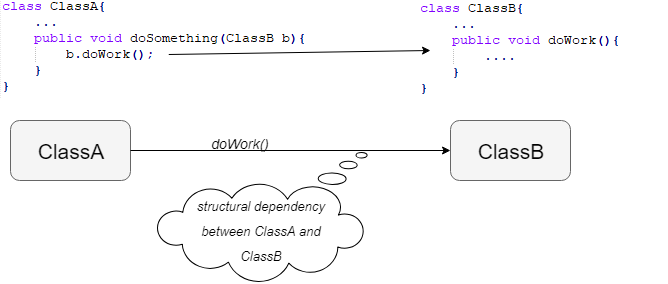
\includegraphics[width=\textwidth]{structural_dep.png}
	\caption{\label{fig:fig}Example of structural dependency between two classes}
     \end{figure}
\end{center}

\end{frame}

%%%%%%%%%%%%%%%%%%%%%%%%%%%%%%%%%%%%%%%%%%%

 \begin{frame}
\frametitle{Logical dependencies}
\begin{block}{Definition}
 Logical dependencies are the result of software history analysis and can reveal relationships that are not present in the source code code (structural dependencies).
\end{block}

\begin{center}
     \begin{figure}
	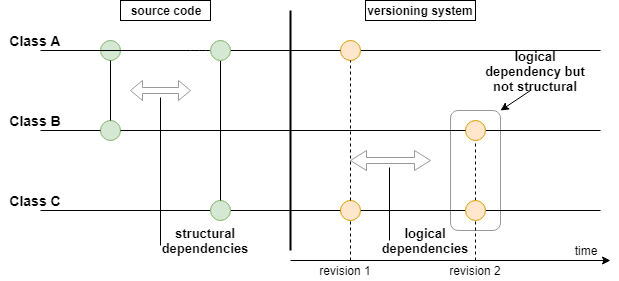
\includegraphics[width=\textwidth]{fig1.png}
	\caption{\label{fig:fig1}Example of logical and structural dependencies}
     \end{figure}
\end{center}

\end{frame}

%%%%%%%%%%%%%%%%%%%%%%%%%%%%%%%%%%%%%%%%%%%

 \begin{frame}
\frametitle{Current status of research}
The current trend recommends that general dependency management methods and tools should also include logical dependencies besides the structural dependencies \footnote{Gustavo Ansaldi Oliva and Marco Aurelio Gerosa. On the interplay between
structural and logical dependencies in open-source software.}, \footnote{Nemitari Ajienka and Andrea Capiluppi. Understanding the interplay between the logical and structural coupling of software classes.}. \\
But there are no strict rules to \textit{filter co-changes into logical dependencies}, other researches filtered co-changes only in order to decrease their number and not to increase their validity.

\end{frame}

%%%%%%%%%%%%%%%%%%%%%%%%%%%%%%%%%%%%%%%%%%

 \begin{frame}
\frametitle{Research content - filter co-changing classes into logical dependencies}
\begin{center}
     \begin{figure}
	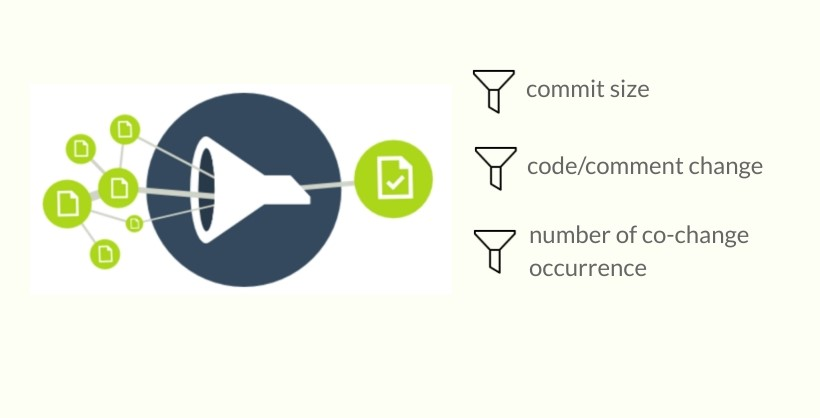
\includegraphics[width=\textwidth]{filter.jpg}
	\caption{\label{fig:fig3}Filters for co-changing classes.}
     \end{figure}
\end{center}
\footnote{Adelina Diana Stana and Ioana Sora. Identifying logical dependencies from co-changing classes. }

\end{frame}
%%%%%%%%%%%%%%%%%%%%%%%%%%%%%%%%%%%%%%%%%%

 \begin{frame}
\frametitle{Research content - refine filter for occurrences of co-changing classes}

\begin{center}
     \begin{figure}
	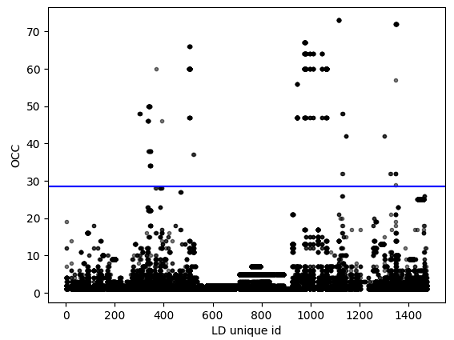
\includegraphics[width= 9.0 cm]{filter_occ.PNG}
	\caption{\label{fig:fig4} Occurrences rates of co-changing classes extracted from one system. }
     \end{figure}
\end{center}

\end{frame}
%%%%%%%%%%%%%%%%%%%%%%%%%%%%%%%%%%%%%%%%%%

 \begin{frame}
\frametitle{Research content - architectural reconstruction}
Use the logical dependencies extracted among structural dependencies in tools for architectural reconstruction to evaluate the improvement.

\end{frame}
%%%%%%%%%%%%%%%%%%%%%%%%%%%%%%%%%%%%%%%%%%

 \begin{frame}
\frametitle{Research content - software metrics}
Compare the number of logical dependencies with metrics and study their connections. Metrics:
\begin{itemize}
	\item  Fan Out - number of other classes referenced by a class.
	\item  Fan In - number of other classes that reference a class.
\end{itemize}

\end{frame}

%%%%%%%%%%%%%%%%%%%%%%%%%%%%%%%%%%%%%%%%%%

 \begin{frame}
\frametitle{Paper: Identifying logical dependencies from co-changing classes}
Filter Thresholds
\begin{itemize}
	\item commit size (cs): the maximum size of commit transactions
which are accepted to generate logical dependencies. The
values for this threshold were 5, 10, 20 and no threshold (infinity).
	\item  number of occurrences (occ): the minimum number of
repeated occurrences for a co-change to be counted as logical
dependency. The values for this threshold were 1, 2, 3 and 4.
	\item with/without taking comments into consideration as valid
change.
\end{itemize}

\end{frame}

%%%%%%%%%%%%%%%%%%%%%%%%%%%%%%%%%%%%%%%%%%

 \begin{frame}
\frametitle{Paper: Identifying logical dependencies from co-changing classes}

\begin{center}
     \begin{figure}
	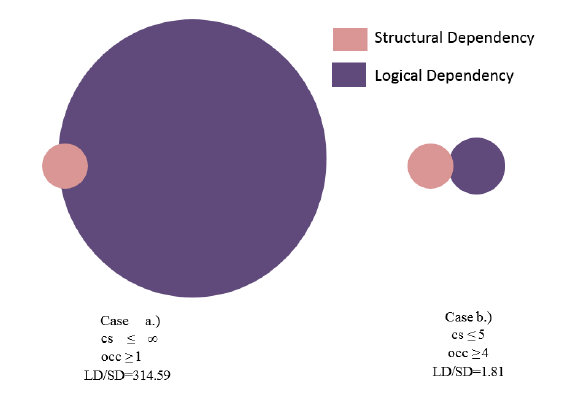
\includegraphics[width= 9.4 cm]{ld_overlapp.PNG}
	\caption{\label{fig:fig5} Logical and structural dependencies overlapping. }
     \end{figure}
\end{center}

\end{frame}

%%%%%%%%%%%%%%%%%%%%%%%%%%%%%%%%%%%%%%%%%

 \begin{frame}
\frametitle{Conclusions}
 \begin{itemize}
        \item  Large number of structural dependencies are not doubled by logical dependencies.
        \item  The most important factors in co-changing classes filtering: commit size (cs) and number of occurrences (occ).
        \item The commit size threshold(cs) influence the size of the extracted co-changes but not their relevance.
        \item Filtering the logical dependencies after occurrences must be made using a dynamically calculated threshold. 
    \end{itemize}
\end{frame}

\end{document}